\documentclass[spanish,letterpaper,oneside]{article}

% Datos del documento
\def\documenttitle {Calibrar para decidir en la formación técnica}
\def\documentsubtitle {Fundamentos para la enseñanza y el aprendizaje I}
\def\documentsubject {Trabajo final · Proyecto educativo por realizar}
\def\documentauthor {Mtro. Martín Jonathan de la Cruz Muñoz}
\def\coursename {Fundamentos para la enseñanza y el aprendizaje I}
\def\coursecode {MAEM}

% Identidad institucional
\def\universityname {Instituto de Investigación, Innovación y Estudios de Posgrado para la Educación del Estado de Nuevo León}
\def\universityfaculty {Maestría en Aprendizaje y Enseñanza de las Matemáticas}
\def\universitydepartment {Fundamentos para la enseñanza y el aprendizaje I}
\def\universitydepartmentimage {img/iiiepe/marca-iiiepe.png}
\def\universitydepartmentimagecfg {height=1.75cm}
\def\universitylocation {Monterrey, Nuevo León}
\def\studentfullname {Mtro. Martín Jonathan de la Cruz Muñoz}
\def\studentid {00874}
\def\studentemail {martin.delacruz@campus.iiiepe.edu.mx}
\def\programperiod {1er tetramestre, marzo--julio de 2026}
\def\programmodality {Modalidad presencial}
\def\programshort {MAEM}

\def\authortable {
  \begin{tabular}{ll}
    \textbf{Alumno:} & \studentfullname \\
    Matrícula: & \studentid \\
    Correo institucional: & \studentemail \\
    Unidad: & \coursename \\
    Programa: & \programshort \\
    Periodo: & \programperiod \\
    & \\
    \multicolumn{2}{l}{Fecha de realización: 13 de octubre de 2026} \\
    \multicolumn{2}{l}{\universitylocation}
  \end{tabular}
}

\input{template}

\usepackage{helvet}
\renewcommand{\familydefault}{\sfdefault}
\usepackage{array}
\usepackage{longtable}
\usepackage{pdflscape}
\usepackage{tikz}
\usepackage[most]{tcolorbox}
\usetikzlibrary{arrows.meta,positioning,calc,fit,backgrounds}

\definecolor{iiiepeNavy}{HTML}{163B5C}
\definecolor{iiiepeBlue}{HTML}{1F6F9F}
\definecolor{iiiepeAqua}{HTML}{20B7A8}
\definecolor{iiiepeOrange}{HTML}{F28C28}
\definecolor{iiiepePaper}{HTML}{F6F8F7}
\definecolor{iiiepeInk}{HTML}{1E2A32}
\def\portraittitlecolor {iiiepeNavy}
\setcitestyle{authoryear,open={(},close={)}}

\newcommand{\insertcoverwatermark}{%
  \AddToShipoutPictureBG*{%
    \begin{tikzpicture}[remember picture,overlay]
      \node[opacity=.09,inner sep=0pt] at (current page.center)
      {\includegraphics[width=.58\paperwidth]{img/iiiepe/logo-puntos.png}};
    \end{tikzpicture}%
  }%
}

\newtcolorbox{reportelecturabox}[1][]{%
  enhanced,breakable,
  colback=iiiepePaper,colframe=iiiepeNavy,
  boxrule=1pt,leftrule=4pt,arc=2pt,
  left=8pt,right=8pt,top=6pt,bottom=6pt,
  before skip=6pt,after skip=10pt,
  fonttitle=\bfseries\color{white},coltitle=white,
  colbacktitle=iiiepeNavy,
  attach boxed title to top left={xshift=8pt,yshift=-2pt},
  boxed title style={colback=iiiepeNavy,colframe=iiiepeNavy,arc=1pt},
  title={Reporte de lectura},#1}

\newtcolorbox{fichalecturabox}[1][]{%
  enhanced,breakable,
  colback=iiiepeAqua!7,colframe=iiiepeAqua!70!iiiepeNavy,
  boxrule=.6pt,arc=1pt,
  left=7pt,right=7pt,top=4pt,bottom=4pt,
  fontupper=\small,before upper={\setstretch{1.0}},
  fonttitle=\bfseries\color{iiiepeNavy},coltitle=iiiepeNavy,
  colbacktitle=iiiepeAqua!7,
  title={Ficha de la lectura},#1}



\usepackage{tabularx,colortbl,pgfplots,enumitem,needspace}\pgfplotsset{compat=1.18}\definecolor{iiiepePale}{HTML}{EEF5F8}
\setlength{\parskip}{5pt}\setlength{\parindent}{0pt}
\begin{document}\insertcoverwatermark\templatePortrait\templatePagecfg\templateFinalcfg\fancyfoot{}\fancyfoot[L]{\scriptsize IIIEPE · MAEM}\fancyfoot[C]{\scriptsize\thepage}\fancyfoot[R]{\scriptsize Trabajo final}\setstretch{1.3}\raggedbottom
\section{Descripción del proyecto}
\textbf{Proyecto propuesto: Calibrar para decidir: matemáticas y uso responsable de un sistema de medición.} Se dirige a preparatoria técnica, especialmente a mantenimiento y mecatrónica, y puede adaptarse a Ingeniería Mecánica, de Sistemas e Industrial mediante mayor profundidad de modelación. Se presenta como proyecto por realizar, posibilidad expresamente contemplada en los lineamientos; no se atribuyen resultados de aplicación.
El propósito es construir y justificar un modelo entre una lectura instrumental y una referencia, interpretar sus errores y proponer una decisión de uso. Desarrolla proporcionalidad, funciones lineales, representaciones tabular y gráfica, medidas de tendencia central y dispersión, unidades y argumentación. El producto es un informe de calibración y una comunicación dirigida a la comunidad escolar. El recurso puede ser un instrumento de baja tensión ya autorizado o una simulación; no se intervienen sistemas eléctricos peligrosos.

\begin{center}
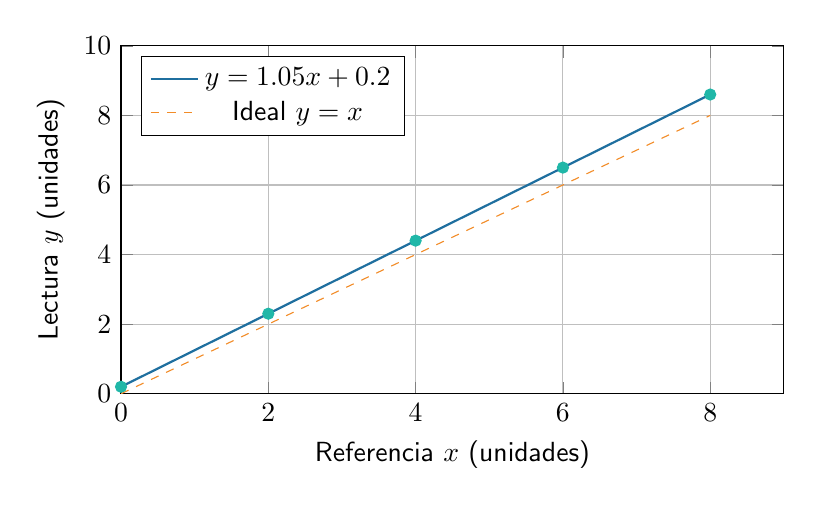
\begin{tikzpicture}\begin{axis}[width=10cm,height=6cm,xlabel={Referencia $x$ (unidades)},ylabel={Lectura $y$ (unidades)},xmin=0,xmax=9,ymin=0,ymax=10,grid=major,legend pos=north west]
\addplot[iiiepeBlue,thick,domain=0:8]{1.05*x+.2};\addlegendentry{$y=1.05x+0.2$}\addplot[iiiepeOrange,dashed,domain=0:8]{x};\addlegendentry{Ideal $y=x$}\addplot[only marks,iiiepeAqua] coordinates {(0,.2)(2,2.3)(4,4.4)(6,6.5)(8,8.6)};\end{axis}\end{tikzpicture}
\end{center}
\section{Necesidad que atiende}
El problema educativo propuesto es la separación entre ejecutar un procedimiento y comprender qué decisión permite sostener. Un estudiante puede obtener una ecuación sin explicar variables, unidades o límites. El proyecto busca hacer visible ese razonamiento mediante una pregunta: ¿cuándo podemos confiar en una lectura para tomar una decisión? Esta necesidad se plantea como hipótesis didáctica que debe contrastarse con un diagnóstico del grupo, no como un déficit ya demostrado.
El trabajo permite vincular la formación técnica con responsabilidad: un modelo debe examinarse y comunicarse sin ocultar error ni incertidumbre. La orientación humanista exige que todos participen en interpretación y decisiones, aunque su familiaridad con instrumentos sea distinta.
\section{Campo formativo y razonamiento matemático}
La resolución de problemas aparece al definir variables y seleccionar un procedimiento; el pensamiento lógico, al verificar relaciones; la argumentación, al justificar el modelo; la representación, al conectar tabla, gráfica y expresión; y la aplicación cotidiana, al interpretar qué tan confiable es una medición. El marco de Saberes y Pensamiento Científico se utiliza como referencia formativa de la consigna; la adaptación a preparatoria debe alinearse después con el programa específico del plantel.


{\small\setstretch{1.1}\renewcommand{\arraystretch}{1.25}
\begin{longtable}{|>{\raggedright\arraybackslash}p{\dimexpr0.3\linewidth-2\tabcolsep-2\arrayrulewidth\relax}|>{\raggedright\arraybackslash}p{\dimexpr0.35\linewidth-2\tabcolsep-2\arrayrulewidth\relax}|>{\raggedright\arraybackslash}p{\dimexpr0.35\linewidth-2\tabcolsep-2\arrayrulewidth\relax}|}\hline
\rowcolor{iiiepePale} \textbf{Referencia $x$} & \textbf{Lectura $y$} & \textbf{Error $y-x$} \\\hline
\endfirsthead
\hline
\rowcolor{iiiepePale} \textbf{Referencia $x$} & \textbf{Lectura $y$} & \textbf{Error $y-x$} \\\hline
\endhead
0 & 0.2 & 0.2 \\\hline
2 & 2.3 & 0.3 \\\hline
4 & 4.4 & 0.4 \\\hline
6 & 6.5 & 0.5 \\\hline
8 & 8.6 & 0.6 \\\hline
\end{longtable}}


Los valores son simulados. En el ejemplo, $y=1.05x+0.2$; la pendiente es 1.05 y el término inicial es 0.2. No es proporcionalidad directa porque el cociente $y/x$ no es constante y $y(0)\ne0$. Si se desea estimar la referencia desde la lectura, $x=(y-0.2)/1.05$. Para una lectura de 6.5, la estimación corregida es 6. La unidad debe definirse al seleccionar el instrumento; la tabla utiliza una escala didáctica sin atribuir magnitud física real.
\section{Metodología sociocrítica y actividades}
Se elige aprendizaje basado en indagación con STEAM como enfoque porque la pregunta requiere diseñar una prueba, obtener datos y contrastar un modelo. La ciencia aporta observación y explicación, la tecnología el recurso de medición, la ingeniería el diseño de prueba, las artes la representación comunicativa y las matemáticas la modelación. La integración se justifica por su función; no exige utilizar todas las disciplinas de forma decorativa.


{\small\setstretch{1.1}\renewcommand{\arraystretch}{1.25}
\begin{longtable}{|>{\raggedright\arraybackslash}p{\dimexpr0.22\linewidth-2\tabcolsep-2\arrayrulewidth\relax}|>{\raggedright\arraybackslash}p{\dimexpr0.78\linewidth-2\tabcolsep-2\arrayrulewidth\relax}|}\hline
\rowcolor{iiiepePale} \textbf{Momento propuesto} & \textbf{Actividad y evidencia} \\\hline
\endfirsthead
\hline
\rowcolor{iiiepePale} \textbf{Momento propuesto} & \textbf{Actividad y evidencia} \\\hline
\endhead
Inicio · 1 sesión & Diagnosticar interpretación de variables y unidades, reconocer condiciones de acceso y acordar pregunta y criterios. Evidencia: predicción individual y plan. \\\hline
Indagación · 2 sesiones & Definir referencias, repetir lecturas y registrar sin alterar datos. Evidencia: tabla, condiciones y observaciones. \\\hline
Modelación · 1 sesión & Construir gráfica, comparar modelos y calcular errores. Evidencia: ecuación y justificación. \\\hline
Comunicación · 1 sesión & Explicar límites y recomendación de uso a compañeros. Evidencia: informe y presentación. \\\hline
Revisión · 1 sesión & Utilizar devoluciones y resolver un caso nuevo. Evidencia: versión corregida y explicación individual. \\\hline
\end{longtable}}


La duración es una propuesta ajustable, no un calendario oficial. El docente guía, modela cuando hace falta y examina decisiones; los estudiantes investigan, representan, argumentan y revisan. Se rotan roles y se ofrece una alternativa de papel para conservar el acceso.
\section{Perspectiva ecológica de Bronfenbrenner}
El microsistema comprende interacciones entre estudiantes, docente y compañeros durante la medición. El mesosistema aparece al conectar tareas escolares con experiencias de taller y comunicación con la familia cuando resulte pertinente. El exosistema incluye disponibilidad de equipos, horarios y decisiones institucionales que condicionan la tarea. El macrosistema incorpora valoraciones sobre matemáticas, tecnología, género y formación profesional. El cronosistema permite observar la transición entre una predicción inicial, una explicación revisada y su transferencia posterior.
La dimensión bioecológica agrega procesos, persona, contexto y tiempo: se analiza cómo la interacción recurrente con datos, símbolos y compañeros sostiene aprendizaje. Bronfenbrenner (1987) ofrece la perspectiva ecológica y Tong y An (2024) advierten sobre reducirla a una lista de contextos. No se atribuye causalidad a un factor sin evidencia.
\section{Evaluación e impacto esperado}
La evaluación inicial recoge explicación y estimación; durante la indagación se revisa registro y control de variables; en el cierre se valora la justificación y una tarea de transferencia. La autoevaluación pide explicar una mejora; la coevaluación contrasta coherencia entre representaciones; la heteroevaluación examina modelación y argumento. El instrumento considera definición de variables, integridad del registro, interpretación del error, accesibilidad y uso de la devolución.
Se espera que los estudiantes distingan relación proporcional y lineal, interpreten un sesgo y comuniquen una decisión con límites. También se busca colaboración y pensamiento crítico. Estos son resultados esperados. Su verificación requerirá evidencias reales comparables y no permitirá afirmar por sí sola un efecto causal del proyecto.
\section{Del dato a una decisión justificable}
En el ejemplo, el error de lectura es $e=y-x=0.05x+0.2$. Existe un sesgo inicial de 0.2 unidades y un componente que crece con la referencia. La ecuación de corrección elimina ambos componentes dentro del modelo construido: para $y=8.6$, $x=(8.6-0.2)/1.05=8$. Esta coincidencia es exacta porque los datos fueron generados con esa relación; no demuestra que un instrumento real responda igual.
Para una aplicación se tomarán repeticiones y se examinarán residuos $r_i=y_i-\widehat y_i$. Si muestran un patrón sistemático, se revisará el modelo o el intervalo; si presentan variación, se analizarán condiciones y precisión del registro. La recomendación de uso debe expresar intervalo, unidad y criterio de aceptación pertinente al instrumento seleccionado. El proyecto no fija una tolerancia normativa sin contar con esa información.

{\small\setstretch{1.1}\renewcommand{\arraystretch}{1.25}
\begin{longtable}{|>{\raggedright\arraybackslash}p{\dimexpr0.22\linewidth-2\tabcolsep-2\arrayrulewidth\relax}|>{\raggedright\arraybackslash}p{\dimexpr0.43\linewidth-2\tabcolsep-2\arrayrulewidth\relax}|>{\raggedright\arraybackslash}p{\dimexpr0.35\linewidth-2\tabcolsep-2\arrayrulewidth\relax}|}\hline
\rowcolor{iiiepePale} \textbf{Criterio} & \textbf{Evidencia de cumplimiento} & \textbf{Decisión de apoyo} \\\hline
\endfirsthead
\hline
\rowcolor{iiiepePale} \textbf{Criterio} & \textbf{Evidencia de cumplimiento} & \textbf{Decisión de apoyo} \\\hline
\endhead
Modelación & Define variables y unidades y distingue función afín de proporcionalidad. & Contrastar el valor inicial con un modelo que pasa por el origen. \\\hline
Registro & Conserva lecturas, referencias, repeticiones y condiciones. & Revisar una fila con el equipo antes de continuar. \\\hline
Argumentación & Relaciona error y límite del modelo con una recomendación. & Pedir un caso fuera del intervalo y discutir por qué no se extrapola. \\\hline
Revisión y participación & Cada integrante explica un cambio entre versiones. & Distribuir preguntas y contrastar explicación individual y producto colectivo. \\\hline
\end{longtable}}
La autoevaluación utiliza estos criterios para identificar un logro y un ajuste; la coevaluación pide señalar una evidencia y formular una pregunta; el docente revisa coherencia y ofrece una acción concreta. La respuesta a la devolución se conserva como parte del producto. El instrumento se propone para la aplicación; no registra desempeños que aún no se han observado.

\section{Reflexión final}
El proyecto concibe el aprendizaje matemático como construcción acompañada de relaciones y argumentos. Las metodologías sociocríticas permiten vincular una pregunta relevante con investigación y participación; su aportación depende de que el contenido sea visible en las decisiones. La perspectiva ecológica evita separar el desempeño de las condiciones y relaciones en que se aprende.
Mi experiencia en administración del conocimiento y del trabajo aporta planificación y verificación. El acercamiento humanista añade atención a quién participa, qué comprende y qué apoyo necesita. El beneficio formativo esperado es que el estudiante pueda decidir responsablemente, explicar su criterio y revisar una conclusión. Mantendría esa exigencia junto con el respeto a ritmos y contextos, sin inventar resultados de una implementación pendiente.

\section{Formación técnica y responsabilidad educativa}
El perfil de Mecatrónica del CONALEP (2025, pp. 1--3) vincula formación integral y juicio ético con diagnóstico, medición y mantenimiento. Esa referencia respalda la pertinencia de relacionar rigor técnico y atención a la persona. En mi perfil docente, la aplicación consiste en pedir razones y decisiones justificadas, con oportunidades de participación y revisión; no en reducir la enseñanza al cumplimiento de una operación.
\needspace{5\baselineskip}\section*{Referencias}
{\setstretch{1.15}\setlength{\parskip}{6pt}
\par\hangindent=1.27cm\hangafter=1  Bronfenbrenner, U. (1987). \textit{La ecología del desarrollo humano}. Paidós.
\par\hangindent=1.27cm Colegio Nacional de Educación Profesional Técnica. (2025). \textit{Perfil de egreso: Profesional Técnico-Bachiller en Mecatrónica. Modelo Académico 2025}. Secretaría Académica. \url{https://www.conalep.edu.mx/sites/default/files/micrositios/perfil_egreso_2025/ElectyElectro/PE25_Mecatr%C3%B3nica.pdf}
\par\hangindent=1.27cm\hangafter=1  Secretaría de Educación Pública. (2022a). \textit{Plan de Estudio para la educación preescolar, primaria y secundaria}. SEP.
\par\hangindent=1.27cm\hangafter=1  Secretaría de Educación Pública. (2022b). \textit{Sugerencias metodológicas para el desarrollo de los proyectos educativos} [Extracto de \textit{Avance del contenido para el libro del docente. Primer grado}, material en proceso de edición, pp. 64--82, 23--24]. SEP.
\par\hangindent=1.27cm\hangafter=1  Secretaría de Educación Pública. (2024). \textit{Programa de estudio para la educación secundaria: Programa sintético de la Fase 6}. SEP.
\par\hangindent=1.27cm\hangafter=1  Tong, P., \& An, I. S. (2024). Review of studies applying Bronfenbrenner’s bioecological theory in international and intercultural education research. \textit{Frontiers in Psychology, 14}, Article 1233925. \url{https://doi.org/10.3389/fpsyg.2023.1233925}
}

\end{document}
